\section{Introduction}

\begin{frame}{\insertsection}{What is topic modeling?}
	\begin{itemize}
		\item Imagine categorizing $100.000+$ documents, manually
	\end{itemize}
	\begin{figure}
		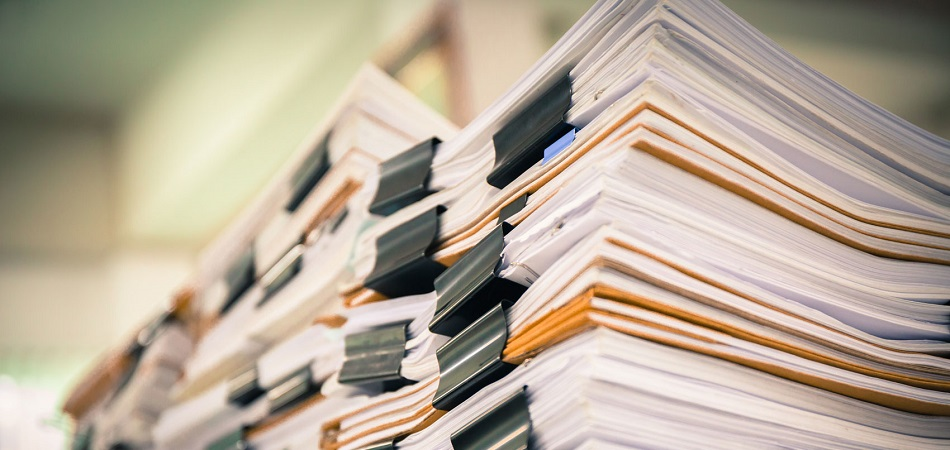
\includegraphics[width=\textwidth]{figures/documents.jpg}
		\let\thefootnote\relax\footnote{\tiny{https://emerj.com/partner-content/ai-based-document-digitization-an-enterprise-guide/}}
	\end{figure}
\end{frame}

\begin{frame}{\insertsection}{What is topic modeling?}
	\begin{itemize}
		\item Topic modeling
  		\begin{itemize}
			\item Data has arisen from a generative process
			\item Discover main themes within a collection of documents.
		\end{itemize}
	\end{itemize}
\end{frame}

\begin{frame}{\insertsection}{What is topic modeling?}
	\begin{figure}
		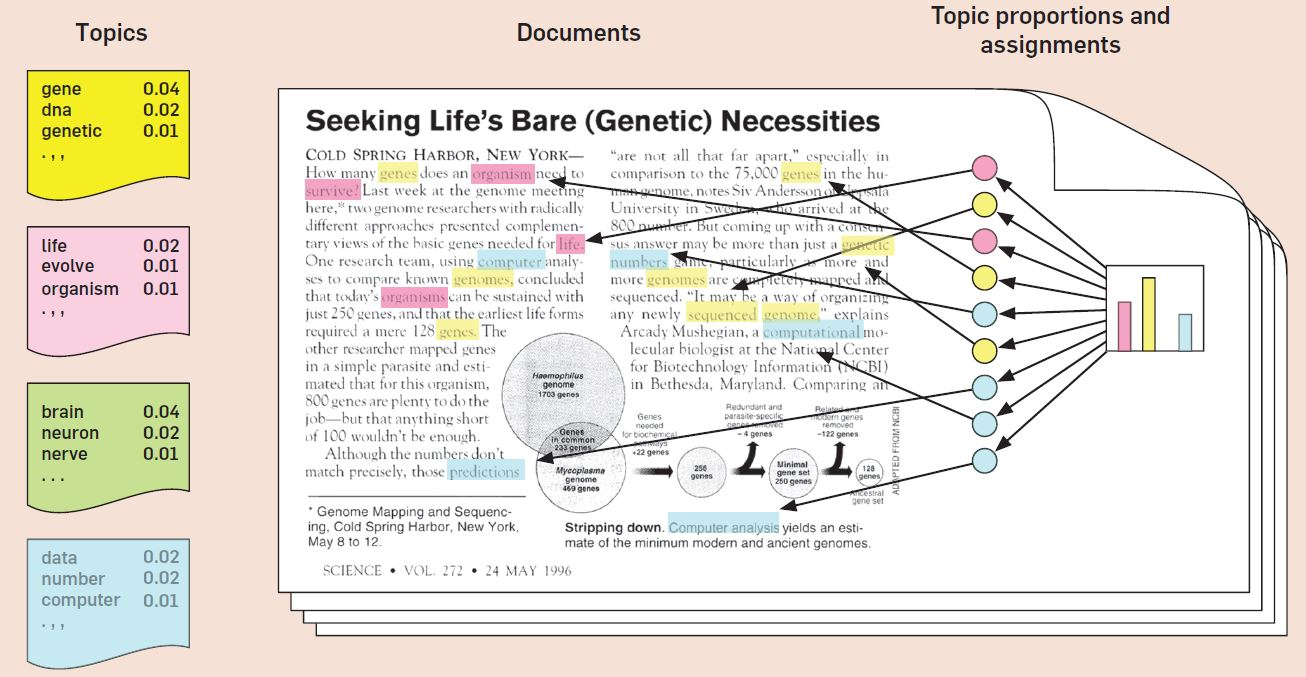
\includegraphics[width=\textwidth]{figures/topic_modeling_visual.JPG}
		\let\thefootnote\relax\footnote{\tiny{http://www.cs.columbia.edu/~blei/papers/Blei2012.pdf}}
	\end{figure}
\end{frame}

\begin{frame}{\insertsection}{Topic modeling using news articles}
	\begin{figure}
		
\includegraphics[width=\textwidth]{figures/danish_newspapers.jpg}
		\let\thefootnote\relax\footnote{\tiny{https://www.fyidenmark.com/denmark-newspapers.html}}
	\end{figure}
\end{frame}

\section{Dataset}

\begin{frame}{\insertsection}{Nordjyske}
	\begin{figure}
		
\includegraphics[width=0.6\textwidth]{figures/nordjyske-medier.png}
		\let\thefootnote\relax\footnote{\tiny{https://addfocus.dk/nordjyske-medier-2/}}
	\end{figure}
	\begin{itemize}
		\item 2017-2019
		\item News articles
		\item Multiple \textbf<2>{metadata} fields
	\end{itemize}
\end{frame}


\begin{frame}{\insertsection}{The three chosen metadata}
	\begin{itemize}
		\item Author
		\item Category
		\item Taxonomy
	\end{itemize}
\end{frame}

\subsection{Author}

\begin{frame}{\insertsubsection}{Metadata description}
	\begin{itemize}
		\item The person who has written the article
		\item $184$ unique authors (after preprocessing)
		\item Example: Peter Tordrup Larsen
	\end{itemize}
\end{frame}


\subsection{Category}

\begin{frame}{\insertsubsection}{Metadata description}
	\begin{itemize}
		\item Newspaper or labels
		\item $34$ unique categories (after preprocessing)
		\item Example: Aalborg-avis or Kultur
	\end{itemize}
\end{frame}


\subsection{Taxonomy}

\begin{frame}{\insertsubsection}{Metadata description}
	\begin{itemize}
		\item A hierarchical structure of topical or geographical information 
		\item $355$ unique taxonomy entries (after preprocessing)
		\item Example: 
		\begin{itemize}
			\item PLACES/Danmark/Nordjylland/Aalborg
			\item TOPICS/Religion/Christianity
		\end{itemize}
	\end{itemize}
\end{frame}

\begin{frame}{\insertsection}{Metadata influence}
	\begin{itemize}
		\item What impact does these metadata have on the topics?
		\item Can it improve the topic quality?
	\end{itemize}
\end{frame}

\section{Models}

\subsection{Latent Dirichlet Allocation}

\begin{frame}{\insertsubsection}{Plate notation}
	\begin{figure}
		\centering
		\resizebox{\textwidth}{!}{%
			\begin{figure}[h]
  \centering
  \resizebox{\columnwidth}{!}{%
	  \begin{tikzpicture}
	    [
	      observed/.style={minimum size=15pt,circle,draw=blue!50,fill=blue!20},
	      unobserved/.style={minimum size=26pt,circle,draw},
	      post/.style={->,>=stealth',semithick},
	    ]
	
	    \node (w-j) [observed] at (0,0) {$W_{d,n}$};
	    \node (z-j) [unobserved] at (-1.5,0) {$Z_{d,n}$};
	    \node (theta) [unobserved] at (-3,0) {$\theta_d$};
	    \node (alpha-hyper) [unobserved, label=above:$\alpha$,left of=theta, node distance=2cm] {};
	    \node (beta-hyper) [unobserved] at (2.75,0) {$\beta_k$};
	    \node (eta-hyper) [unobserved, label=above:$\eta$, ,right of=beta-hyper, node distance=2cm] {};
	    
	    \path
	    (z-j) edge [post] (w-j)
	    (alpha-hyper) edge [post] (theta)
	    (theta) edge [post] (z-j)
	    (beta-hyper) edge [post] (w-j)
	    (eta-hyper) edge [post] (beta-hyper)
	    ;
	    
	    \node [draw,fit=(w-j) (theta), inner sep=14pt] (plate-context) {};
	    \node [above right] at (plate-context.south west) {$D$};
	    \node [draw,fit=(w-j) (z-j), inner sep=10pt] (plate-token) {};
	    \node [above right] at (plate-token.south west) {$N$};
	    \node [draw,fit=(beta-hyper) (beta-hyper), inner sep=17pt] (plate-context) {};
	    \node [above right] at (plate-context.south west) {$K$};
	  \end{tikzpicture}
  }
	\caption{Plate notation for \gls{lda}.}
	\label{fig:standard_lda}
\end{figure}
		}
	\end{figure}
	\begin{itemize}
		\item $\alpha$ and $\eta$ are topic hyperparameters
		\item $\theta_d$ and $\beta_k$ are the document-topic and topic-word distribution
		\item $Z_{d,n}$ is the topic assignment 
	\end{itemize}
	\let\thefootnote\relax\footnote{\tiny{All pieces are random variables}}
\end{frame}


\begin{frame}{\insertsubsection}{Dirichlet distribution}
	\begin{itemize}
		\item Dirichlet distribution
	\end{itemize}
	\begin{figure}
		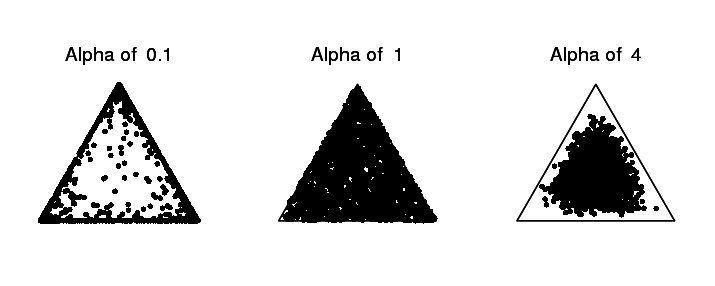
\includegraphics[width=\textwidth]{figures/dirich.png}
		\let\thefootnote\relax\footnote{\tiny{https://mollermara.com/blog/lda/}}
	\end{figure}
\end{frame}

\subsection{Author-Topic Model}

\begin{frame}{\insertsubsection}{Plate notation}
	\begin{columns}
		\begin{column}{0.45\textwidth}
			\begin{figure}
				\resizebox{\textwidth}{!}{%
				\begin{tikzpicture}
	 [
	   observed/.style={minimum size=15pt,circle,draw=blue!50,fill=blue!20, node distance=2cm},
	   unobserved/.style={minimum size=26pt,circle,draw, node distance=2cm},
	   post/.style={->,>=stealth',semithick},
	 ]
	
	 \node (w-j) [observed] at (0,0) {$W_{d,n}$};
	 \node (z-j) [unobserved, above of = w-j] {$Z_{d,n}$};
	 \node (theta) [unobserved, above of = z-j] {$\theta_d$};
	 \node (alpha-hyper) [unobserved, label=above:$\alpha$,left of=theta] {};
	 \node (beta-hyper) [unobserved, left of = w-j, node distance=2.5cm] {$\beta_k$};
	 \node (eta-hyper) [unobserved, label=above:$\eta$, left of=beta-hyper] {};
	 
	 \path
	 (z-j) edge [post] (w-j)
	 (alpha-hyper) edge [post] (theta)
	 (theta) edge [post] (z-j)
	 (beta-hyper) edge [post] (w-j)
	 (eta-hyper) edge [post] (beta-hyper)
	 ;
	 
	 \node [draw,fit=(w-j) (theta), inner sep=14pt] (plate-context) {};
	 \node [below right] at (plate-context.north west) {$D$};
	 \node [draw,fit=(w-j) (z-j), inner sep=10pt] (plate-token) {};
	 \node [below right] at (plate-token.north west) {$N$};
	 \node [draw,fit=(beta-hyper) (beta-hyper), inner sep=17pt] (plate-context) {};
	 \node [above right] at (plate-context.south west) {$K$};
\end{tikzpicture}
			}
			\caption*{The LDA model}
			\end{figure}
		\end{column}
		\begin{column}{0.45\textwidth}
			\begin{figure}
				\resizebox{\textwidth}{!}{%
					\begin{tikzpicture}
	[
	observed/.style={minimum size=26pt,circle,draw=blue!50,fill=blue!20},
	unobserved/.style={minimum size=26pt,circle,draw},
	post/.style={->,>=stealth',semithick},
	]
	
	\node (w-j) [observed] at (0,0) {$W_{d,n}$};
	\node (z-j) [unobserved, above of= w-j, node distance=2.5cm] {$Z_{d,n}$};
	\node (author_obs) [observed, above of= z-j, node distance=1.5cm] {$a_d$};
	\node (author_dist) [unobserved, left of=z-j, node distance=2.5cm] {$\theta_a$};
	\node (alpha-hyper) [unobserved, label=above:$\alpha$, left of=category_dist, node distance=2cm] {};
	\node (beta-hyper) [unobserved, left of = w-j, node distance=2.5cm] {$\beta_k$};
	\node (eta-hyper) [unobserved, label=above:$\eta$, left of=beta-hyper, node distance=2cm] {};
	
	\path
	(z-j) edge [post] (w-j)
	(alpha-hyper) edge [post] (author_dist)
	(author_obs) edge [post] (z-j)
	(author_dist) edge [post] (z-j)
	(beta-hyper) edge [post] (w-j)
	(eta-hyper) edge [post] (beta-hyper)
	;
	
	\node [draw,fit=(w-j) (author_obs), inner sep=14pt] (plate-context) {};
	\node [below right] at (plate-context.north west) {$D$};
	
	\node [draw,fit=(w-j) (z-j), inner sep=10pt] (plate-token) {};
	\node [below right] at (plate-token.north west) {$N$};
	
	\node [draw,fit=(beta-hyper) (beta-hyper), inner sep=17pt] (plate-context) {};
	\node [above right] at (plate-context.south west) {$K$};
	
	\node [draw,fit=(author_dist) (author_dist), inner sep=17pt] (plate-context) {};
	\node [above right] at (plate-context.south west) {$A$};
\end{tikzpicture}
				}
				\caption*{The author-topic model}
			\end{figure}
		\end{column}
	\end{columns}
\end{frame}

\begin{frame}{\insertsubsection}{Plate notation}
		\begin{columns}
		\begin{column}{0.38\textwidth}
			\begin{figure}
				\resizebox{\textwidth}{!}{%
					\begin{tikzpicture}
	 [
	   observed/.style={minimum size=15pt,circle,draw=blue!50,fill=blue!20, node distance=2cm},
	   unobserved/.style={minimum size=15pt,circle,draw, node distance=2cm},
	   post/.style={->,>=stealth',semithick},
	 ]
	
	 \node (z-j) [unobserved] at (0,0) {$Z_{d,n}$};
	 \node (theta) [unobserved, left of = z-j] {$\theta_d$};
	 \node (alpha-hyper) [unobserved, label=above:$\alpha$,left of=theta] {};
	 
	 \path
	 (alpha-hyper) edge [post] (theta)
	 (theta) edge [post] (z-j)
	 ;
	 
	 \node [draw,fit=(w-j) (theta), inner sep=14pt] (plate-context) {};
	 \node [below right] at (plate-context.north west) {$D$};
	 \node [draw,fit=(w-j) (z-j), inner sep=10pt] (plate-token) {};
	 \node [below right] at (plate-token.north west) {$N$};
\end{tikzpicture}
				}
				\caption*{The LDA model}
			\end{figure}
		\end{column}
		\begin{column}{0.52\textwidth}
			\begin{figure}
				\resizebox{\textwidth}{!}{%
					\begin{tikzpicture}
	[
	observed/.style={minimum size=15pt,circle,draw=blue!50,fill=blue!20, node distance=2cm},
	unobserved/.style={minimum size=15pt,circle,draw, node distance=2cm},
	post/.style={->,>=stealth',semithick},
	]
	
	\node (z-j) [unobserved] at (0,0) {$Z_{d,n}$};
	\node (author_obs) [observed, right of= z-j] {$a_d$};
	\node (author_dist) [unobserved, left of=z-j, node distance=2.5cm] {$\theta_a$};
	\node (alpha-hyper) [unobserved, label=above:$\alpha$, left of=author_dist] {};
	
	\path
	(alpha-hyper) edge [post] (author_dist)
	(author_obs) edge [post] (z-j)
	(author_dist) edge [post] (z-j)
	;
	
	\node [draw,fit=(w-j) (author_obs), inner sep=14pt] (plate-context) {};
	\node [below left] at (plate-context.north east) {$D$};
	
	\node [draw,fit=(w-j) (z-j), inner sep=10pt] (plate-token) {};
	\node [below left] at (plate-token.north east) {$N$};
	
	\node [draw,fit=(author_dist) (author_dist), inner sep=17pt] (plate-context) {};
	\node [above right] at (plate-context.south west) {$A$};
\end{tikzpicture}
				}
				\caption*{The author-topic model}
			\end{figure}
		\end{column}
	\end{columns}
\end{frame}


\subsection{Category-Topic Model}
\begin{frame}{\insertsubsection}{Plate notation}
	\begin{columns}
		\begin{column}{0.45\textwidth}
			\begin{figure}
				\resizebox{\textwidth}{!}{%
					\begin{tikzpicture}
	[
	observed/.style={minimum size=15pt,circle,draw=blue!50,fill=blue!20, node distance=2cm},
	unobserved/.style={minimum size=15pt,circle,draw, node distance=2cm},
	post/.style={->,>=stealth',semithick},
	]
	
	\node (z-j) [unobserved] at (0,0) {$Z_{d,n}$};
	\node (author_obs) [observed, right of= z-j] {$a_d$};
	\node (author_dist) [unobserved, left of=z-j, node distance=2.5cm] {$\theta_a$};
	\node (alpha-hyper) [unobserved, label=above:$\alpha$, left of=author_dist] {};
	
	\path
	(alpha-hyper) edge [post] (author_dist)
	(author_obs) edge [post] (z-j)
	(author_dist) edge [post] (z-j)
	;
	
	\node [draw,fit=(w-j) (author_obs), inner sep=14pt] (plate-context) {};
	\node [below left] at (plate-context.north east) {$D$};
	
	\node [draw,fit=(w-j) (z-j), inner sep=10pt] (plate-token) {};
	\node [below left] at (plate-token.north east) {$N$};
	
	\node [draw,fit=(author_dist) (author_dist), inner sep=17pt] (plate-context) {};
	\node [above right] at (plate-context.south west) {$A$};
\end{tikzpicture}
				}
				\caption*{Author-topic}
			\end{figure}
		\end{column}
		\begin{column}{0.45\textwidth}
			\begin{figure}
				\resizebox{\textwidth}{!}{%
					\begin{tikzpicture}
	[
	observed/.style={minimum size=15pt,circle,draw=blue!50,fill=blue!20, node distance=2cm},
	unobserved/.style={minimum size=15pt,circle,draw, node distance=2cm},
	post/.style={->,>=stealth',semithick},
	]
	
	\node (z-j) [unobserved] at (0,0) {$Z_{d,n}$};
	\node (category_obs) [observed, right of= z-j] {$c_d$};
	\node (category_dist) [unobserved, left of=z-j, node distance=2.5cm] {$\theta_c$};
	\node (alpha-hyper) [unobserved, label=above:$\alpha$, left of=category_dist] {};
	
	\path
	(alpha-hyper) edge [post] (category_dist)
	(category_obs) edge [post] (z-j)
	(category_dist) edge [post] (z-j)
	;
	
	\node [draw,fit=(w-j) (category_obs), inner sep=14pt] (plate-context) {};
	\node [below left] at (plate-context.north east) {$D$};
	
	\node [draw,fit=(w-j) (z-j), inner sep=10pt] (plate-token) {};
	\node [below left] at (plate-token.north east) {$N$};
	
	\node [draw,fit=(category_dist) (category_dist), inner sep=17pt] (plate-context) {};
	\node [above right] at (plate-context.south west) {$C$};
\end{tikzpicture}
				}
				\caption*{Category-topic}
			\end{figure}
		\end{column}
	\end{columns}
\end{frame}

\begin{frame}{\insertsection}{}
	\begin{itemize}
		\item How does author and category influence the topics found by the model?
	\end{itemize}
\end{frame}
